\documentclass{beamer}
\usepackage{tikz}
\usetikzlibrary{arrows.meta, decorations.pathreplacing, calc}

% ------------------------------------------------------------------
% Theme colors & styles: blkline / blkfill / accentline / accentfill /
% lbl / flow. Assumed to already exist in your master preamble — delete
% this block if dropping these frames into that file.
% ------------------------------------------------------------------
\definecolor{blkline}{HTML}{375775}
\definecolor{blkfill}{HTML}{EAF0F7}
\definecolor{accentline}{HTML}{B5651D}
\definecolor{accentfill}{HTML}{FBEEDD}
\tikzset{
  lbl/.style={text=black},
  flow/.style={-{Stealth[length=2.2mm]}, thick},
  loadedbox/.style={draw=blkline, fill=blkfill, thick},
  extbox/.style={draw=blkline, fill=blkfill!35, thick, dashed},
}

% \bw, \rh shared by every frame
\def\bw{1.0}
\def\rh{0.62}
\def\regx{0.7}
\def\regy{4.3}
\def\memx{5.2}
\def\memy{3.0}

\begin{document}

% ==================================================================
% LDRH — zero-extended halfword
% ==================================================================
\begin{frame}{LDRH: Loading a Halfword (Zero-Extended)}
\centering
\resizebox{0.92\textwidth}{!}{%
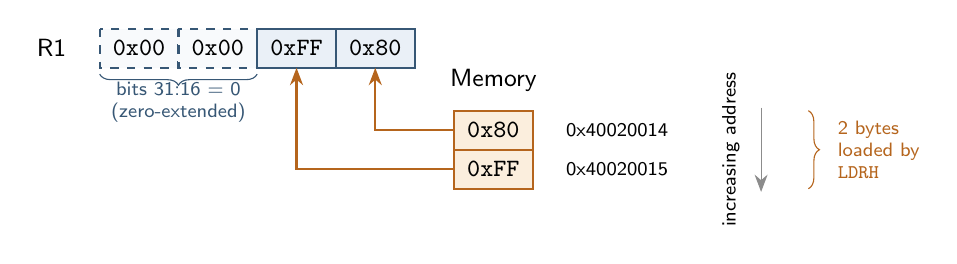
\begin{tikzpicture}[x=10mm, y=8mm]

% --- Register R1: byte3..byte0 left to right; only byte1,byte0 loaded ---
\foreach \p/\val/\loaded in {0/{0x00}/0, 1/{0x00}/0, 2/{0xFF}/1, 3/{0x80}/1}{
  \pgfmathsetmacro{\x}{\regx+\p*\bw}
  \ifnum\loaded=1
    \draw[loadedbox] (\x,\regy) rectangle ({\x+\bw},{\regy-\rh});
  \else
    \draw[extbox] (\x,\regy) rectangle ({\x+\bw},{\regy-\rh});
  \fi
  \node[font=\ttfamily\small] at ({\x+\bw/2},{\regy-\rh/2}) {\val};
}
\node[lbl, anchor=east, font=\sffamily\small] at ({\regx-0.3},{\regy-\rh/2}) {R1};

% under-brace: zero-extended upper half
\draw[decorate, decoration={brace, amplitude=4pt, mirror}, draw=blkline]
    ({\regx},{\regy-\rh-0.1}) -- ({\regx+2*\bw},{\regy-\rh-0.1});
\node[lbl, font=\sffamily\scriptsize, text=blkline, align=center]
    at ({\regx+\bw},{\regy-\rh-0.55}) {bits 31:16 = 0\\(zero-extended)};

% --- Memory: 2 bytes, low address on top (LSB) ---
\foreach \i/\val/\addr in {0/{0x80}/{0x40020014}, 1/{0xFF}/{0x40020015}}{
  \pgfmathsetmacro{\y}{\memy-\i*\rh}
  \draw[draw=accentline, fill=accentfill, thick] (\memx,\y) rectangle ({\memx+\bw},{\y-\rh});
  \node[font=\ttfamily\small] at ({\memx+\bw/2},{\y-\rh/2}) {\val};
  \node[lbl, anchor=west, font=\sffamily\scriptsize] at ({\memx+\bw+0.3},{\y-\rh/2}) {\addr};
}
\node[lbl, anchor=south, font=\sffamily\small] at ({\memx+\bw/2},{\memy+0.15}) {Memory};

% --- Arrows: 2 bytes flow up into byte1,byte0 ---
\draw[flow, draw=accentline] (\memx,{\memy-0*\rh-\rh/2}) -| ({\regx+3*\bw+\bw/2},{\regy-\rh});
\draw[flow, draw=accentline] (\memx,{\memy-1*\rh-\rh/2}) -| ({\regx+2*\bw+\bw/2},{\regy-\rh});

% --- Address axis + brace ---
\def\axisx{9.1}
\draw[-{Stealth[length=2.2mm]}, draw=black!45]
    ({\axisx},{\memy+0.05}) -- ({\axisx},{\memy-2*\rh-0.05});
\node[lbl, anchor=south, rotate=90, font=\sffamily\scriptsize]
    at ({\axisx-0.15},{\memy-1*\rh}) {increasing address};
\draw[decorate, decoration={brace, amplitude=4pt}, draw=accentline]
    ({\axisx+0.6},{\memy}) -- ({\axisx+0.6},{\memy-2*\rh});
\node[lbl, anchor=west, align=left, font=\sffamily\scriptsize, text=accentline]
    at ({\axisx+0.85},{\memy-1*\rh}) {2 bytes\\loaded by\\\texttt{LDRH}};

\end{tikzpicture}%
}
\end{frame}

% ==================================================================
% LDRB — zero-extended byte
% ==================================================================
\begin{frame}{LDRB: Loading a Byte (Zero-Extended)}
\centering
\resizebox{0.92\textwidth}{!}{%
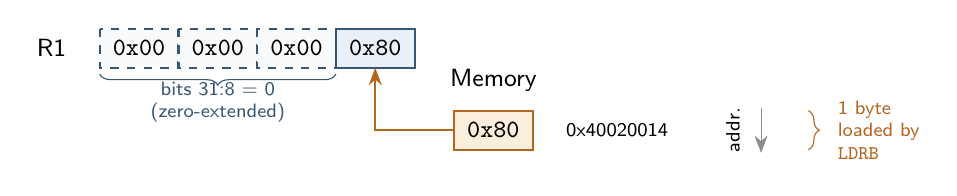
\begin{tikzpicture}[x=10mm, y=8mm]

% --- Register R1: only byte0 loaded ---
\foreach \p/\val/\loaded in {0/{0x00}/0, 1/{0x00}/0, 2/{0x00}/0, 3/{0x80}/1}{
  \pgfmathsetmacro{\x}{\regx+\p*\bw}
  \ifnum\loaded=1
    \draw[loadedbox] (\x,\regy) rectangle ({\x+\bw},{\regy-\rh});
  \else
    \draw[extbox] (\x,\regy) rectangle ({\x+\bw},{\regy-\rh});
  \fi
  \node[font=\ttfamily\small] at ({\x+\bw/2},{\regy-\rh/2}) {\val};
}
\node[lbl, anchor=east, font=\sffamily\small] at ({\regx-0.3},{\regy-\rh/2}) {R1};

% under-brace: zero-extended upper 3 bytes
\draw[decorate, decoration={brace, amplitude=4pt, mirror}, draw=blkline]
    ({\regx},{\regy-\rh-0.1}) -- ({\regx+3*\bw},{\regy-\rh-0.1});
\node[lbl, font=\sffamily\scriptsize, text=blkline, align=center]
    at ({\regx+1.5*\bw},{\regy-\rh-0.55}) {bits 31:8 = 0\\(zero-extended)};

% --- Memory: 1 byte ---
\draw[draw=accentline, fill=accentfill, thick] (\memx,\memy) rectangle ({\memx+\bw},{\memy-\rh});
\node[font=\ttfamily\small] at ({\memx+\bw/2},{\memy-\rh/2}) {0x80};
\node[lbl, anchor=west, font=\sffamily\scriptsize] at ({\memx+\bw+0.3},{\memy-\rh/2}) {0x40020014};
\node[lbl, anchor=south, font=\sffamily\small] at ({\memx+\bw/2},{\memy+0.15}) {Memory};

% --- Arrow: 1 byte flows up into byte0 ---
\draw[flow, draw=accentline] (\memx,{\memy-\rh/2}) -| ({\regx+3*\bw+\bw/2},{\regy-\rh});

% --- Address axis + brace ---
\def\axisx{9.1}
\draw[-{Stealth[length=2.2mm]}, draw=black!45]
    ({\axisx},{\memy+0.05}) -- ({\axisx},{\memy-\rh-0.05});
\node[lbl, anchor=south, rotate=90, font=\sffamily\scriptsize]
    at ({\axisx-0.15},{\memy-0.5*\rh}) {addr.};
\draw[decorate, decoration={brace, amplitude=4pt}, draw=accentline]
    ({\axisx+0.6},{\memy}) -- ({\axisx+0.6},{\memy-\rh});
\node[lbl, anchor=west, align=left, font=\sffamily\scriptsize, text=accentline]
    at ({\axisx+0.85},{\memy-0.5*\rh}) {1 byte\\loaded by\\\texttt{LDRB}};

\end{tikzpicture}%
}
\end{frame}

% ==================================================================
% LDRSH — sign-extended halfword
% ==================================================================
\begin{frame}{LDRSH: Loading a Halfword (Sign-Extended)}
\centering
\resizebox{0.92\textwidth}{!}{%
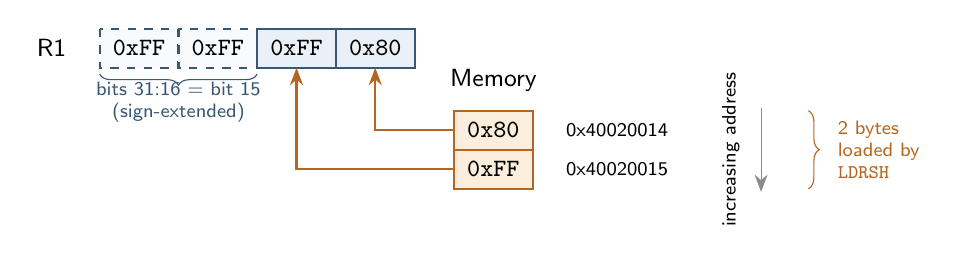
\begin{tikzpicture}[x=10mm, y=8mm]

% --- Register R1: byte1,byte0 loaded; byte3,byte2 replicate the sign bit ---
\foreach \p/\val/\loaded in {0/{0xFF}/0, 1/{0xFF}/0, 2/{0xFF}/1, 3/{0x80}/1}{
  \pgfmathsetmacro{\x}{\regx+\p*\bw}
  \ifnum\loaded=1
    \draw[loadedbox] (\x,\regy) rectangle ({\x+\bw},{\regy-\rh});
  \else
    \draw[extbox] (\x,\regy) rectangle ({\x+\bw},{\regy-\rh});
  \fi
  \node[font=\ttfamily\small] at ({\x+\bw/2},{\regy-\rh/2}) {\val};
}
\node[lbl, anchor=east, font=\sffamily\small] at ({\regx-0.3},{\regy-\rh/2}) {R1};

% under-brace: sign-extended upper half
\draw[decorate, decoration={brace, amplitude=4pt, mirror}, draw=blkline]
    ({\regx},{\regy-\rh-0.1}) -- ({\regx+2*\bw},{\regy-\rh-0.1});
\node[lbl, font=\sffamily\scriptsize, text=blkline, align=center]
    at ({\regx+\bw},{\regy-\rh-0.55}) {bits 31:16 = bit 15\\(sign-extended)};

% --- Memory: 2 bytes, same halfword 0xFF80 as LDRH (bit 15 = 1) ---
\foreach \i/\val/\addr in {0/{0x80}/{0x40020014}, 1/{0xFF}/{0x40020015}}{
  \pgfmathsetmacro{\y}{\memy-\i*\rh}
  \draw[draw=accentline, fill=accentfill, thick] (\memx,\y) rectangle ({\memx+\bw},{\y-\rh});
  \node[font=\ttfamily\small] at ({\memx+\bw/2},{\y-\rh/2}) {\val};
  \node[lbl, anchor=west, font=\sffamily\scriptsize] at ({\memx+\bw+0.3},{\y-\rh/2}) {\addr};
}
\node[lbl, anchor=south, font=\sffamily\small] at ({\memx+\bw/2},{\memy+0.15}) {Memory};

% --- Arrows: 2 bytes flow up into byte1,byte0 ---
\draw[flow, draw=accentline] (\memx,{\memy-0*\rh-\rh/2}) -| ({\regx+3*\bw+\bw/2},{\regy-\rh});
\draw[flow, draw=accentline] (\memx,{\memy-1*\rh-\rh/2}) -| ({\regx+2*\bw+\bw/2},{\regy-\rh});

% --- Address axis + brace ---
\def\axisx{9.1}
\draw[-{Stealth[length=2.2mm]}, draw=black!45]
    ({\axisx},{\memy+0.05}) -- ({\axisx},{\memy-2*\rh-0.05});
\node[lbl, anchor=south, rotate=90, font=\sffamily\scriptsize]
    at ({\axisx-0.15},{\memy-1*\rh}) {increasing address};
\draw[decorate, decoration={brace, amplitude=4pt}, draw=accentline]
    ({\axisx+0.6},{\memy}) -- ({\axisx+0.6},{\memy-2*\rh});
\node[lbl, anchor=west, align=left, font=\sffamily\scriptsize, text=accentline]
    at ({\axisx+0.85},{\memy-1*\rh}) {2 bytes\\loaded by\\\texttt{LDRSH}};

\end{tikzpicture}%
}
\end{frame}

% ==================================================================
% LDRSB — sign-extended byte
% ==================================================================
\begin{frame}{LDRSB: Loading a Byte (Sign-Extended)}
\centering
\resizebox{0.92\textwidth}{!}{%
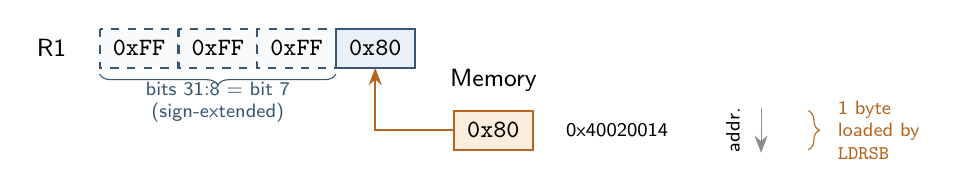
\begin{tikzpicture}[x=10mm, y=8mm]

% --- Register R1: only byte0 loaded; byte3,byte2,byte1 replicate the sign bit ---
\foreach \p/\val/\loaded in {0/{0xFF}/0, 1/{0xFF}/0, 2/{0xFF}/0, 3/{0x80}/1}{
  \pgfmathsetmacro{\x}{\regx+\p*\bw}
  \ifnum\loaded=1
    \draw[loadedbox] (\x,\regy) rectangle ({\x+\bw},{\regy-\rh});
  \else
    \draw[extbox] (\x,\regy) rectangle ({\x+\bw},{\regy-\rh});
  \fi
  \node[font=\ttfamily\small] at ({\x+\bw/2},{\regy-\rh/2}) {\val};
}
\node[lbl, anchor=east, font=\sffamily\small] at ({\regx-0.3},{\regy-\rh/2}) {R1};

% under-brace: sign-extended upper 3 bytes
\draw[decorate, decoration={brace, amplitude=4pt, mirror}, draw=blkline]
    ({\regx},{\regy-\rh-0.1}) -- ({\regx+3*\bw},{\regy-\rh-0.1});
\node[lbl, font=\sffamily\scriptsize, text=blkline, align=center]
    at ({\regx+1.5*\bw},{\regy-\rh-0.55}) {bits 31:8 = bit 7\\(sign-extended)};

% --- Memory: 1 byte, same source byte 0x80 as LDRB (bit 7 = 1) ---
\draw[draw=accentline, fill=accentfill, thick] (\memx,\memy) rectangle ({\memx+\bw},{\memy-\rh});
\node[font=\ttfamily\small] at ({\memx+\bw/2},{\memy-\rh/2}) {0x80};
\node[lbl, anchor=west, font=\sffamily\scriptsize] at ({\memx+\bw+0.3},{\memy-\rh/2}) {0x40020014};
\node[lbl, anchor=south, font=\sffamily\small] at ({\memx+\bw/2},{\memy+0.15}) {Memory};

% --- Arrow: 1 byte flows up into byte0 ---
\draw[flow, draw=accentline] (\memx,{\memy-\rh/2}) -| ({\regx+3*\bw+\bw/2},{\regy-\rh});

% --- Address axis + brace ---
\def\axisx{9.1}
\draw[-{Stealth[length=2.2mm]}, draw=black!45]
    ({\axisx},{\memy+0.05}) -- ({\axisx},{\memy-\rh-0.05});
\node[lbl, anchor=south, rotate=90, font=\sffamily\scriptsize]
    at ({\axisx-0.15},{\memy-0.5*\rh}) {addr.};
\draw[decorate, decoration={brace, amplitude=4pt}, draw=accentline]
    ({\axisx+0.6},{\memy}) -- ({\axisx+0.6},{\memy-\rh});
\node[lbl, anchor=west, align=left, font=\sffamily\scriptsize, text=accentline]
    at ({\axisx+0.85},{\memy-0.5*\rh}) {1 byte\\loaded by\\\texttt{LDRSB}};

\end{tikzpicture}%
}
\end{frame}

\end{document}
